\documentclass[a4paper,11pt]{article}
\usepackage{graphicx}
\usepackage{amsmath}
\usepackage{graphics}
\usepackage[T1]{fontenc}
\usepackage[utf8]{inputenc}
\usepackage{lmodern}
\usepackage[top=1in, bottom=1in, left=1in, right=1in]{geometry}

\title{SNS Andreev Bound States}
\author{Ben Rosemeyer}

\begin{document}

\maketitle
\tableofcontents

\begin{abstract}
We discuss the bound states of an SNS structure in 1D using the Anreev Approximation and beyond to the full Hamiltonian solution. Numerical solutions are also provided for various phase differences of the two superconductors ($\phi = \phi_L-\phi_R$). Finally, we discuss possibile magnetic effects that these states can exhibit.
\end{abstract}

\section*{Setup and Boundary Conditions}
We begin by cosidering a SNS structure with order parameter: \\

  \[\Delta(x)= \left\{
  \begin{array}{lr}
     \Delta_0 e^{i\phi_L}& : x < -L/2\\
     0 & : -L/2 < x < L/2  0\\
     \Delta_0 e^{i\phi_R} & : x > L/2 
  \end{array}
\right.
\]
The Hamiltonian for such a system is: \\
\begin{equation}
\left( \begin{array}{cc}
\mathcal{H}_0 & \Delta(x) \\
\Delta^*(x) & -\mathcal{H}_0 
 \end{array} \right)
 \left( \begin{array}{cc}
\psi_1 \\
\psi_2
 \end{array} \right) = E
  \left( \begin{array}{cc}
\psi_1 \\
\psi_2
 \end{array} \right)
\end{equation}
With $\mathcal{H}_0 = -\frac{\hbar^2}{2m}\frac{d^2}{dx^2} - \mu$.

The Hamiltonian is written in the Bogoliubov-de Gennes (BdG) representation with $\psi_1$ thought of as a "particle" ($c_k c^\dagger_k$) and $\psi_2$ a "hole" ($c_k c_k + h.c.$).

The bound states of this system (ie. those with energy $|E|<\Delta_0$) have solutions in the normal part:
\begin{equation}
\Psi_{e\pm} = e^{\pm ik_e x}\left( \begin{array}{cc}
1 \\
0
 \end{array} \right), \quad\quad
\Psi_{h\pm} =  e^{\pm ik_h x}\left( \begin{array}{cc}
0 \\
1
 \end{array} \right)
\end{equation}
$k_{e/h} = k_f\sqrt{1\pm E/\mu}$, $k_f = \sqrt{2m\mu/\hbar}$.
The superconducter solutions:
\begin{equation}
\Psi^{L/R}_{+\pm} = e^{\pm ik_+ x}\left( \begin{array}{cc}
u e^{i\phi_{L/R}/2}\\
v e^{-i\phi_{L/R}/2}
 \end{array} \right), \quad
 \Psi^{L/R}_{-\pm} e^{\pm ik_- x}\left( \begin{array}{cc}
v e^{i\phi_{L/R}/2} \\
u e^{-i\phi_{L/R}/2}
 \end{array} \right)
\end{equation}

$k_{\pm}= k_f\sqrt{1\pm i\sqrt{(\Delta_0/\mu)^2-(E/\mu)^2}}$ \\
$u/v = \sqrt{\bigg(1\pm i \sqrt{(\Delta_0/E)^2-1}\bigg)/2}$   \hspace{3cm} NOTE: $u/v\Rightarrow\pm$ NOT division

In what follows we consider two cases: \\
1) Right moving: $A \Psi_{e+} + B \Psi_{h+}$ in normal section, $D\Psi^R_{++}$ in right sc, and $C\Psi^L_{-+}$ in left sc \\
2) Left moving: $A \Psi_{e-} + B \Psi_{h-}$ in normal section, $D\Psi^R_{--}$ in right sc, and $C\Psi^L_{+-}$ in left sc.

We determine the constants $A-D$ with continuous boundary conditios at $\pm L/2$. We can write these boundary conditions in matrix form: \\
{\bf CASE 1}
\begin{equation}
 \left( \begin{array}{cccc}
  \Psi_{e+}(-L/2) & \Psi_{h+}(-L/2) & -\Psi^L_{-+}(-L/2) & 0\\
  \Psi_{e+}(L/2) & \Psi_{h+}(L/2) & 0 & -\Psi^R_{++}(-L/2)
 \end{array} \right)
 \left( \begin{array}{cccc}
A \\
B \\
C \\
D \\
 \end{array} \right) = 0
\end{equation}
{\bf CASE 2}
\begin{equation}
 \left( \begin{array}{cccc}
  \Psi_{e-}(-L/2) & \Psi_{h-}(-L/2) & -\Psi^L_{+-}(-L/2) & 0\\
  \Psi_{e-}(L/2) & \Psi_{h-}(L/2) & 0 & -\Psi^R_{--}(-L/2)
 \end{array} \right)
 \left( \begin{array}{cccc}
A \\
B \\
C \\
D \\
 \end{array} \right) = 0
\end{equation}
These equations have non trivial solutions only if $det(\hat{M})=0$

\section*{Andreev Approximation}
In the Andreev approximation we make the assumption that $\Delta_0$ and the energies E are small compared to $\mu$ which result in the following taylor expansions for the momentums in the normal section: \\
\begin{equation}
k_{e/h} = k_f(1 \pm E/(2\mu)) = k_f \pm \lambda,\quad\quad\lambda = E/(\hbar v_f),\quad\quad \hbar v_f = 2\mu/k_f
\end{equation}

In the superconductors we expand for $x^2 = (\Delta^2-E^2)/\mu^2$: \\
\begin{equation}
k_{\pm} = k_f(1\pm x/2) = kf \pm \lambda_s,\quad\quad \lambda_s = \sqrt{\Delta_0^2-E^2}/(\hbar v_f)
\end{equation}

With this result, there is a term like $e^{ik_f}$ in all the rows of the boundary condition matrix. If we divide the two equations for the left and right boundaries respectively for case 1: \\
LEFT: $(A/B)e^{-i\lambda L} = (v/u) e^{i\phi_L}$\\
RIGHT: $(A/B)e^{i\lambda L} = (u/v) e^{i\phi_R}$ \\
combining these two results in the following transcendental equation:
\begin{equation}
e^{2i\lambda L + i(\phi)} = \frac{u^2}{v^2}
\end{equation}
Similary, the result for case 2 is:
\begin{equation}
e^{2i\lambda L - i(\phi)} = \frac{u^2}{v^2}
\end{equation}
$\phi=\phi_L-\phi_R$. Solutions to this are plotted with the solutions found without the Andreev Approximation in the next section
\section*{Solution to Hamiltonian}
Here we present numeric results for the bound state energies by solving the full boundary condition matrix in equation 4 and 5. We also include the results of the energies for the Andreev Approximation.

\section*{Discussion}
The results are interpreted in the following way. \\
I) Longer normal section results in more bound states\\
II) Phase difference between the superconductors can be used to tune the number and energies of the states \\
III) There are states which exist for L=0 as long as there is a phase difference in the superconductor (ie $\phi\ne 0$). These are seen as zero bias peaks in the conductance (ZBCP) in superconductors with phase boundaries. \\
IIII) With an applied field (in the pauli limit) these levels will be split which could exclude certain spin states from existing. (spin polarized ZBCP?)

\begin{figure}
  \begin{center}
    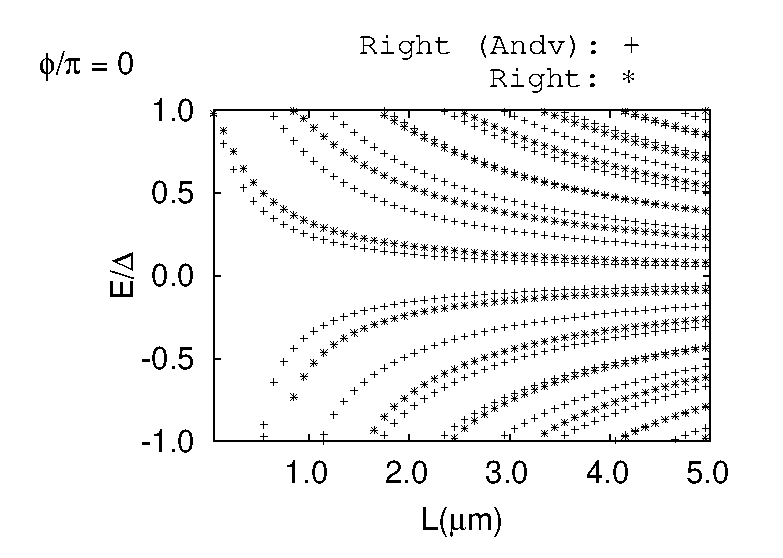
\includegraphics{levels_with_L_0pi.eps}
    \label{fig:}
    \caption{Energies vs length of the normal region for $\phi=0$. Both right and left moving solutions are identical here. + symbols are solution to the Andreev Approximation, while * are full solutions to the boundary matrix}
  \end{center}
\end{figure}

\begin{figure}
  \begin{center}
    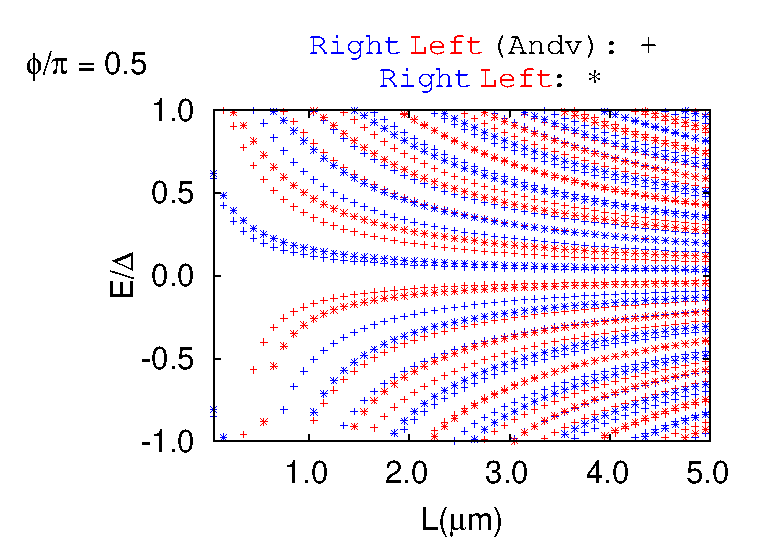
\includegraphics{levels_with_L_pi2.eps}
    \label{fig:}
    \caption{Energies vs length of the normal region for $\phi=\pi/2$. energies for the right moving case are blue, left moving are red. + symbols are solution to the Andreev Approximation, while * are full solutions to the boundary matrix}
  \end{center}
\end{figure}

\begin{figure}
  \begin{center}
    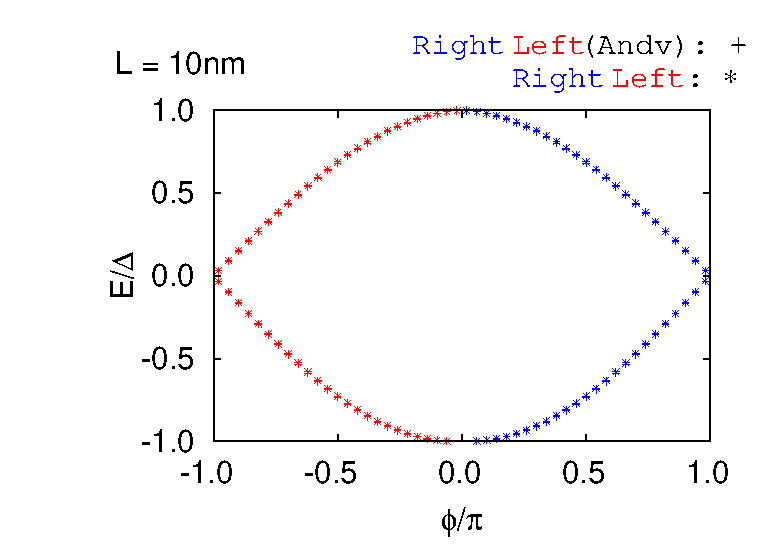
\includegraphics{levels_with_p_10L.eps}
    \label{fig:}
    \caption{Energies vs $\phi$ for normal length $10 nm$. energies for the right moving case are blue, left moving are red. + symbols are solution to the Andreev Approximation, while * are full solutions to the boundary matrix}
  \end{center}
\end{figure}

\begin{figure}
  \begin{center}
    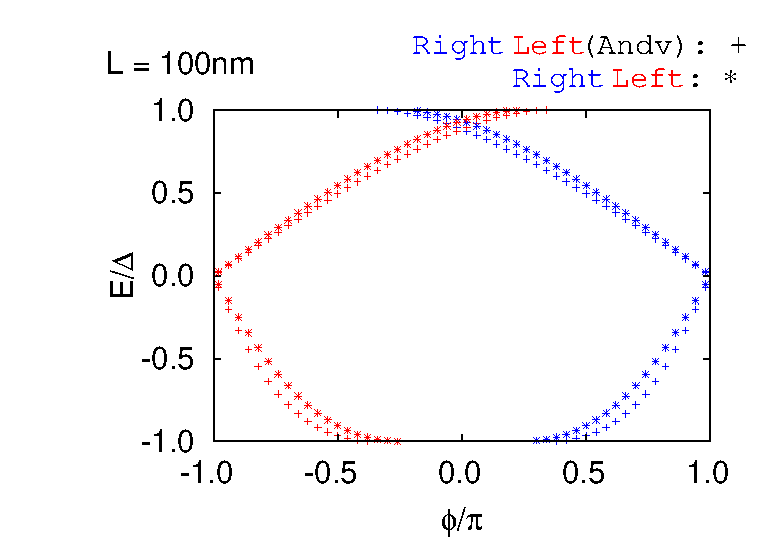
\includegraphics{levels_with_p_100L.eps}
    \label{fig:}
    \caption{Energies vs $\phi$ for normal length $100 nm$. energies for the right moving case are blue, left moving are red. + symbols are solution to the Andreev Approximation, while * are full solutions to the boundary matrix}
  \end{center}
\end{figure}

\begin{figure}
  \begin{center}
    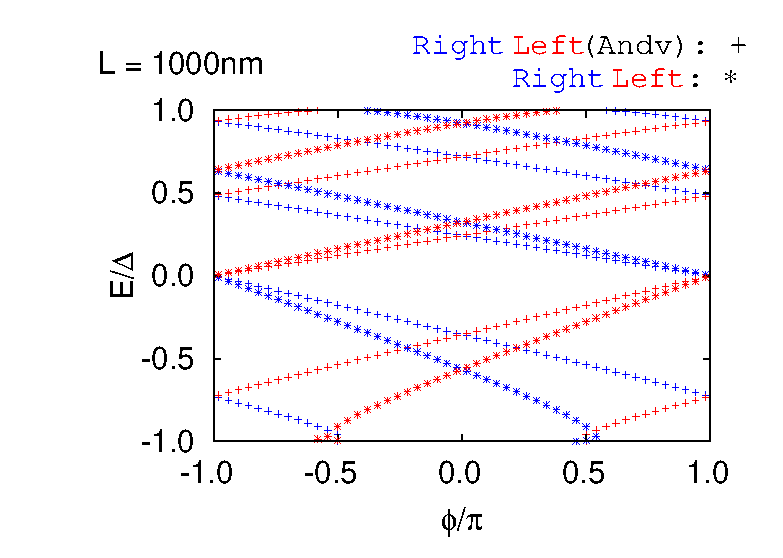
\includegraphics{levels_with_p_1000L.eps}
    \label{fig:}
    \caption{Energies vs $\phi$ for normal length $1000 nm$. energies for the right moving case are blue, left moving are red. + symbols are solution to the Andreev Approximation, while * are full solutions to the boundary matrix}
  \end{center}
\end{figure}


\end{document}
